\documentclass{article}
\usepackage{graphicx}
\usepackage[a4paper, left=2cm, right=2cm, top=2.5cm, bottom=2cm]{geometry}
\usepackage[small]{titlesec}
\usepackage{subcaption} 
\usepackage[italian]{babel}
\usepackage[hidelinks]{hyperref}
\usepackage{listings}
\usepackage{sectsty}
%\usepackage[light]{CormorantGaramond}
\usepackage{fancyhdr}
\usepackage{footnote}
\usepackage{tgadventor}
\usepackage{titling}
\usepackage{graphicx}
\usepackage{tcolorbox}
\usepackage{multirow}
\usepackage{booktabs}
\usepackage{makecell}
\usepackage{algpseudocode}
\usepackage{algorithm}
\usepackage{mathtools}
\usepackage{amssymb}


\setlength{\droptitle}{-5em}   % regola la posizione del titolo
\pretitle{\begin{center}\LARGE}   % imposta la dimensione della font del titolo
\posttitle{\end{center}}
%\lstset{language=C}
\renewcommand\bfdefault{bx}
\sectionfont{\fontsize{20.74}{15}\selectfont}
\subsectionfont{\fontsize{17.28}{15}\selectfont}
\subsubsectionfont{\fontsize{12}{15}\selectfont}
\title{}

\author{}
\date{\today}


\begin{document}
\pagestyle{fancy}
\fancyhf{}
%\rhead{\thepage}
%\lhead{\rightmark}
\rfoot{\thepage}
\lhead{\quad \leftmark}
\rhead{ \quad \rightmark}

\renewcommand{\headrulewidth}{0.2pt}



\begin{titlepage}
    \begin{figure}[t]
        \centering
        
\includegraphics[width=0.7\textwidth]{im/logo_sapienza_new.png}
        \label{fig:logo}
    \end{figure}    
    \null\vfill
    \begin{center}
      {\Huge Appunti di Basi Dati Modulo I} \\[2cm]
      {\Large Colacel Alexandru Andrei}
    \end{center}
    \vfill\null
    \renewcommand{\abstractname}{Disclaimer}

    
    
    \begin{abstract}  
    
    \hrulefill


    Le fonti sono le "Hand Notes" del prof. Perelli tradotte in italiano, appunti presi dalle slides della prof. De Marsico ed eventuali e-mail.\\
    \textbf{Nota: è vietata assolutamente la vendita di questo materiale in qualsiasi forma senza il mio consenso.} 
    \hrulefill
    \end{abstract}
  \end{titlepage}


\pagebreak
\tableofcontents

\pagebreak


\section{Lemma della Chiusura}
Sia $R$ uno schema e sia $F$ un insieme di dipendenze funzionali definite su $R$. Si ha che:\par 
\[X \rightarrow Y \in F^{A} \Longleftrightarrow Y \subseteq X^{+}\]

\subsection{Dimostrazione $\Rightarrow$}

Dato $X$ $\rightarrow$ $Y \in F^{A}$, per la regola della decomposizione, otteniamo:
\[X \rightarrow A \in F^{A}, \quad \forall A \in Y\]

e quindi, per definizione di $X^{+}$, otteniamo che: 

\[A \in X^{+}, \quad \forall A \in Y  \]

che significa: 

\[Y \subseteq X^{+}\]



\subsection{Dimostrazione $\Leftarrow$}
Dato: 
\[Y \subseteq X^{+}\]
si ottiene che: 

\[X \rightarrow A \in F^{A} \quad \forall A \in Y\]

che implica, per la regola dell'unione, che: 

\[X \rightarrow Y \in F^{A}\]


\pagebreak
\section{Teorema $F^{+}$ = $F^{A}$}

Dato uno schema $R$ e un insieme $F$ di dipendenze funzionali definite su $R$, si ha che:
\[ F^{+} = F^{A}\]


\subsection{Dimostrazione $F^{A} \subseteq F^{+}$}
Prendiamo $X \rightarrow Y \in F^{A}$, noi dobbiamo provare che $X \rightarrow Y \in F^{+}$ per induzione con $n$ numero di applicazioni degli assiomi di Armstrong.
\begin{itemize}
  \item \textbf{Caso base} (n = 0): se $X \rightarrow Y \in F^{A}$ senza aver applicato alcun assioma di Armstrong, allora l'unica possibilità è che:
  \[X \rightarrow Y \in F \subseteq F^{+}\]

  \item \textbf{Ipotesi induttiva forte:} ogni dipendenza funzionale in $F^{A}$ ottenuta da $F$
  applicando k $\leq$ n assiomi di Armstrong è anche in $F^{+}$:
  \begin{center}
    $X \rightarrow Y \in F^{A}$ tramite $k \leq n$ assiomi $\Rightarrow X \rightarrow Y \in F^{+}$
  \end{center}
  \item \textbf{Passo induttivo:} è necessario dimostrare che se $X \rightarrow Y \in F^{A}$ dopo aver applicato $n +1$ assiomi di Armstrong, allora $ X \rightarrow Y \in F^{+}$.\par
  È possibile ritrovarsi in uno dei seguenti tre casi:
  \begin{enumerate}
    \item Se l'$(n + 1)$-esimo assioma applicato è l'assioma di \textbf{riflessività}, allora l'unica possibilità è che:

    \[X \rightarrow Y \in F^{A} \Leftrightarrow Y \subseteq X \subseteq R\]

    Dunque, poiché, $Y \subseteq X \subseteq R$, per ogni istanza legale di $R$ si ha che:

    \[\forall t_1, t_2 \in r_{1}, t_1[X] = t_2[X] \Rightarrow t_1[Y] = t_2[Y]\]
    da cui ne segue automaticamente che $X \rightarrow Y \in F^{+}$
    \item Se l'$(n + 1)$-esimo assioma applicato è l'assioma di \textbf{aumento}, allora è obbligatoriamente necessario che:
    \begin{itemize}
      \item $\exists V, W \subseteq R \, | \, \exists V \rightarrow W \in F_{A}$, ottenuta applicando $j \leq n$ assiomi di Armstrong\\

      \item $\exists Z \subseteq R \, | \, X := VZ, \, Y := WZ$\\
    \end{itemize}
      Affinché si abbia che:

      \[Z \subseteq R, \, V \rightarrow W \Rightarrow VZ \rightarrow WZ = X \rightarrow Y \in F^{A}\]

      Siccome per ipotesi induttiva si ha $V \rightarrow W \in F^{A} \Rightarrow V \rightarrow W \in F^{+}$ e siccome $Z \subseteq Z \Rightarrow Z \rightarrow Z \in F^{+}$, si vede facilmente che: 
      \begin{figure}[hbt]
        \begin{center}
            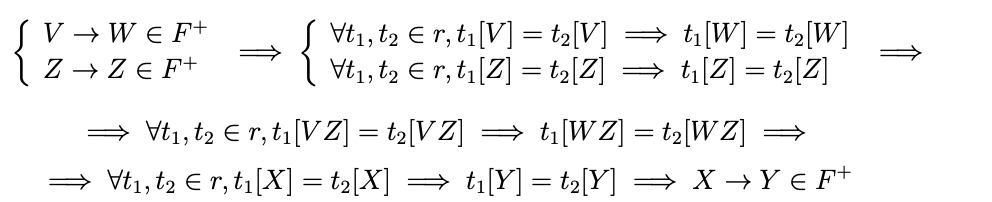
\includegraphics[width=0.8\textwidth,keepaspectratio]{{im/1}}
        \end{center}
        \end{figure}
        \pagebreak
      \item Se l'$(n + 1)$-esimo assioma applicato è l'assioma di \textbf{transitività}, allora è obbligatoriamente necessario che $\exists X \rightarrow Z, Z \rightarrow Y \in F^{A}$, ottenute con $k \leq n$ assiomi di Armstrong, affinché si abbia che:

      \[X \rightarrow Z \in F^{A} \lor Z \rightarrow Y \in F^{A} \Rightarrow X \rightarrow Y \in F^{A}\]

      Siccome per ipotesi induttiva $X \rightarrow Z \in F^{A} \Rightarrow X \rightarrow Z \in F^{+}$ e $Z \rightarrow Y \in F^{A} \Rightarrow Z \rightarrow Y \in F^{+}$, si vede facilmente che:
      \begin{figure}[hbt]
        \begin{center}
            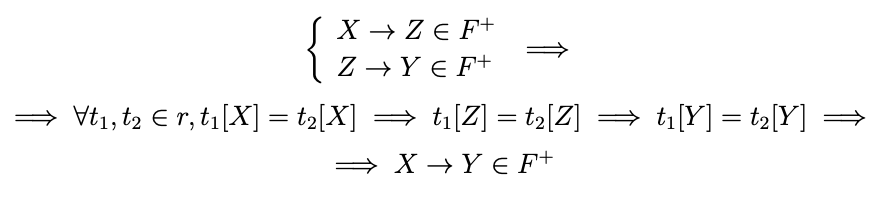
\includegraphics[width=0.7\textwidth,keepaspectratio]{{im/2}}
        \end{center}
        \end{figure}
  \end{enumerate}
\end{itemize}

\pagebreak
\subsection{Dimostrazione $F^{+} \subseteq F^{A}$}
\begin{figure}[hbt]
  \begin{center}
      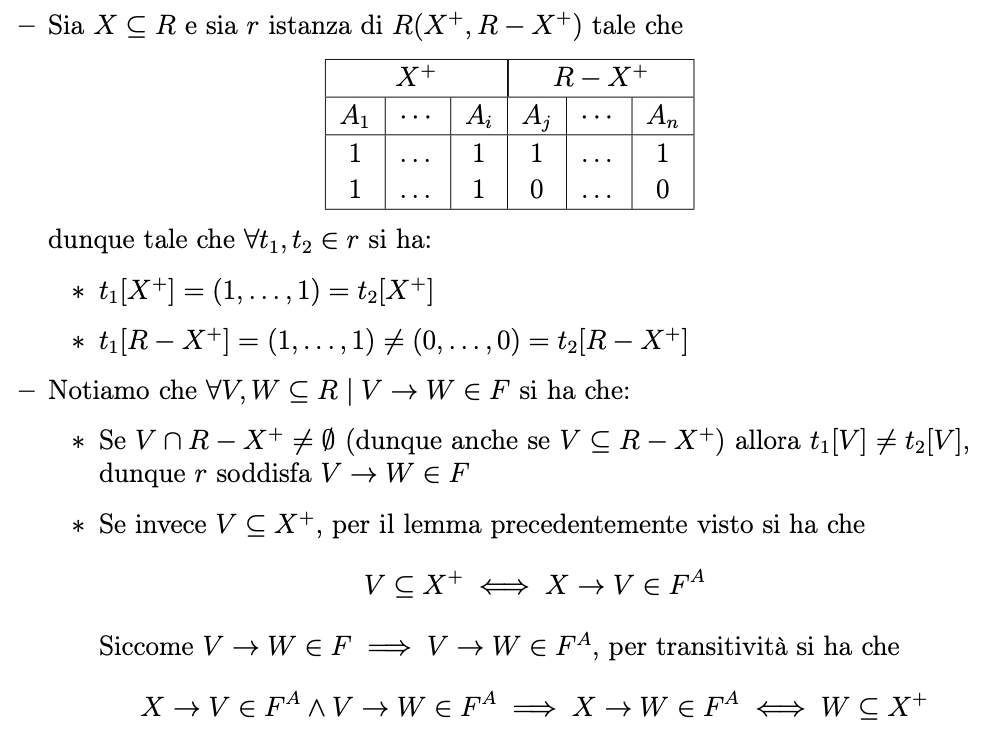
\includegraphics[width=0.75\textwidth,keepaspectratio]{{im/3}}
  \end{center}
  \end{figure}
  \begin{figure}[hbt]
    \begin{center}
        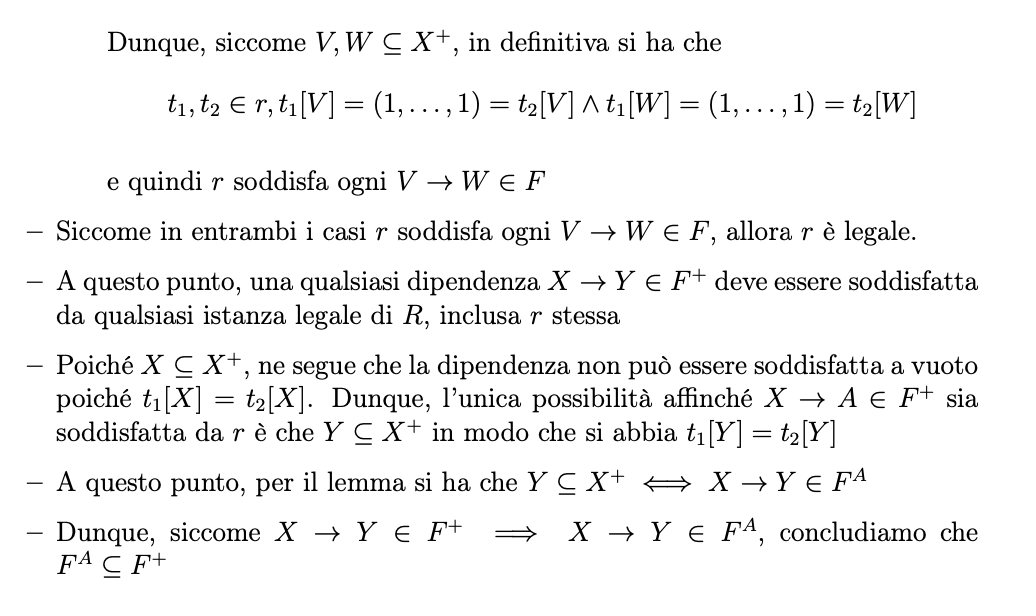
\includegraphics[width=0.8\textwidth,keepaspectratio]{{im/4}}
    \end{center}
    \end{figure}
    
    \begin{tcolorbox}[colback=white!20!white,colframe=green!70!black, title=Nota]
      Poiché $F^{+} = F^{A}$, per calcolare $F^{+}$ ci basta applicare gli assiomi di Armstrong sulle dipendenze in $F$ in modo da trovare $F^{A}$. \par Tuttavia, calcolare $F^{+} = F^{A}$ richiede tempo esponenziale, quindi $O(2^{nk})$: considerando anche solo l'assioma di riflessività, siccome ogni possibile sottoinsieme di $R$ genera una dipendenza e siccome i sottoinsiemi possibili di $R$ sono $2^{|R|}$, allora ne segue che $|F^{+}| >> 2^{|R|}$.
    \end{tcolorbox}

    




\pagebreak
\section{Chiusura di X}
\texttt{Input}:
\begin{itemize}
  \item Relazione $R$
  \item Dipendenze Funzionali $F$
  \item Insieme $X \subseteq R$
\end{itemize}
\texttt{Output}: $X^{+}$\\

\begin{algorithm}
  \caption{Closure Algorithm}  
    \begin{algorithmic}[1]
  \State $Z \gets X$
  \State $S \gets \{A \mid \exists Y \rightarrow V \in F, A \in V \land Y \subseteq Z\}$
  \While{$S \not\subseteq Z$}
    \State $Z \gets Z \cup S$
    \State $S \gets \{A \mid \exists Y \rightarrow V \in F, A \in V \land Y \subseteq Z\}$
  \EndWhile
  \State \textbf{return} $Z$
  \end{algorithmic}
\end{algorithm}
Tale algoritmo viene eseguito in tempo polinomiale, ossia $On^{k}$

\subsection{Teorema: L'algoritmo computa $X_{F}^{+}$}
Il teorema calcola correttamente la chiusura di un insieme di attributi X rispetto ad un insieme F di dipendenze funzionali.

\textbf{Dimostrazione}:\par
Denotiamo:\par

\[Z_{0}, Z_{1}, \dots, Z_{i}, \dots \]
\[S_{0}, S_{1}, \dots, S_{i}, \dots\]

Indichiamo con $Z_{0}$ il valore iniiale di $Z (Z_{0} = X)$ e con $Z_{i}$ e $S_{i}$, $i \geq 1$ i valori di $Z$ ed $S$ dopo l'$i$-esima esecuzione del corpo del ciclo, infatti notiamo che $Z_{i} \subseteq Z_{i+1}$, per ogni $i$.\par
Sia $j$ tale che $S_{j} \subseteq Z_{j}$ (cioè,  $Z_{j}$ è l'output di $Z$ quando l'algoritmo termina); proveremo che:

\[A \in Z_{j} \Leftrightarrow A \in X^{+} \]
\begin{itemize}
  \item Dimostriamo per induzione su $i$ che $Z_{f} \subseteq X^{+}$
  \begin{itemize}
    \item Caso base dell'induzione: i = 0.\par Alla 0-esima iterazione del while (ossia prima di esso) si ha $Z_{0} = X$ e $X \subseteq X^{+}$

    \item Ipotesi induttiva: Per ogni $i \in\mathbb{N}$ si ha che $Z_i \subseteq X^+$

    \item \textbf{Passo induttivo} ($i > 0$):
    Dato $A \in Z_{i+1} = Z_i \cup S_i$, si ha che $A \in Z_i \lor A \in S_i$. \par 
    Dunque, si possono verificare due casi:
    \begin{itemize}
      \item $\text{Se } A \in Z_i, \text{ allora per ipotesi } A \in Z_i \subseteq X^+.$
      \item $\text{Se } A \in S_i, \text{ allora } \exists Y \rightarrow V \in F \text{ tale che } A \in V \subseteq R, Y \subseteq Z_i.$\par
      $\text{Siccome per ipotesi } Z_i \subseteq X^+ \text{ e } Y \subseteq Z_i, \text{ allora } Y \subseteq Z_i \subseteq X^+ \iff X \rightarrow Y \in F^A \text{ e } Y \rightarrow V \in F \implies Y \rightarrow V \in F^A, \text{ quindi per transitività si ha che:}$

      \[X \rightarrow Y, Y \rightarrow V \in F^A \implies X \rightarrow V \in F^A \iff V \subseteq X^+\]
      Dunque,si ha che $A \in V \subseteq X^+$
      \item $\text{Siccome in entrambi i casi } A \in Z_{i+1} \implies A \in X^+, \text{ allora concludiamo che } Z_{i+1} \subseteq X^+$.

    \end{itemize}
    
  \end{itemize}
  \pagebreak
  \item Dimostriamo ora che $X^{+} \subseteq Z_{i}$:\par
  \begin{itemize}
    \item Sia $X \subseteq R$ e sia $r$ istanza di $R(Z_{i}, R-Z_{i})$. 
    \begin{table}[ht]
      \centering
      \begin{tabular}{|c|c|c|c|c|c|}
      \hline
      \multicolumn{3}{|c|}{$Z_{i}$} & \multicolumn{3}{c|}{$R - Z_{i}$} \\
      \hline
      $A_1$ & $\dots$ & $A_{i}$ & $A_{j}$ & $\dots$  & $A_{n}$ \\
      \hline
      $1$ & $\dots$ & $1$ & $1$ & $\dots$  & $1$ \\
      \hline
      $1$ & $\dots$ & $1$ & $0$ & $\dots$  & $0$ \\
      \hline
      \end{tabular}
  \end{table}

  dunque tale che per $t_{1}, t_{2} \in r$ si ha:
  \begin{itemize}
    \item $t_{1}[Z_{i}] = (1, \dots, 1) = t_{2}[Z_{i}]$
    \item $t_{1}[R - Z_{i}] = (1, \dots, 1) \neq (0, \dots, 0) = t_{2}[R - Z_{i}]$
  \end{itemize}
    \item Notiamo che $\forall V, W \subseteq R$ | $V \rightarrow W \in F$ si ha che:
    \begin{itemize}
      \item Se $V \cap (R - Z_i) \neq \emptyset$ (quindi anche se $V \subseteq R - Z_i$) allora $t1[V] \neq t2[V]$, quindi $r$ soddisfa $V \rightarrow W \in F$
      \item Se invece $V \subseteq Z_i$, allora $W \subseteq S_f$, poiché per come viene calcolato $S_f$, si ha che:\par
      $V \rightarrow W \in F$, $V \subseteq Z_i$, $B \in W \subseteq R \Rightarrow B \in S_f \Rightarrow W \subseteq S_f$\par
      e quindi, siccome $S_f \subseteq Z_i$ è la condizione che termina l'algoritmo, allora $W \subseteq S_f \subseteq Z_i$
      \item Siccome $V, W \subseteq Z_i$, in definitiva si ha che\par $t1, t2 \in r$, $t1[V] = (1, \dots, 1) = t2[V]$ e $t1[W] = (1, \dots, 1) = t2[W]$,\par e quindi $r$ soddisfa $V \rightarrow W \in F$
    \end{itemize}
    \item Siccome in entrambi i casi $r$ soddisfa ogni $V \rightarrow W \in F$, allora $r$ è legale.
    \item A questo punto, dato $A \in X^+$, si ha che $X \rightarrow A \in F^A = F^+$ deve essere soddisfatta da qualsiasi istanza legale di $R$, inclusa $r$ stessa.
    \item Poiché $X = Z_0 \subseteq Z_i$, ne segue che la dipendenza non può essere soddisfatta a vuoto poiché $t1[X] = t2[X]$. Dunque, l'unica possibilità affinché $X \rightarrow A \in F^+$ sia soddisfatta da $r$ è $A \in Z_i$ in modo che si abbia $t1[A] = t2[A]$.
    \item Dunque, siccome $A \in X^+ \Rightarrow A \in Z_i$, concludiamo che $X^+ \subseteq Z_i$.
  
  \end{itemize}
\end{itemize}

\pagebreak
\section{Lemma: Inclusione delle chiusure}
Dato uno schema $R$ e due insiemi $F$ e $G$ di dipendenze funzionali su $R$, si ha che:\par 

\[F \subseteq G^+ \Leftrightarrow F^+ \subseteq G^+\]

\subsection{Dimostrazione}
\begin{itemize}
  \item Denotiamo come $G \xrightarrow{\text{A}} F$ la possibilità di ottenere F partendo da G applicando una determinata quantità di assiomi di Armstrong.
  \item  Ricordando che $G^A$ è l'insieme di tutte le dipendenze funzionali ottenibile applicando assiomi di Armstrong su $G$, allora:\par

  \[G \xrightarrow{\text{A}} F \Leftrightarrow \forall X \rightarrow Y \in F, \text{ si ha } X \rightarrow Y \in G^A = G^+ \Leftrightarrow F \subseteq G^+\]

  \item Siccome $F \subseteq G \Leftrightarrow G \xrightarrow{\text{A}} F$, per definizione di $F^A = F^+$ si ha che:

  \[F \subseteq G^+ \Rightarrow G \xrightarrow{\text{A}} F \xrightarrow{\text{A}} F^A = F^+ \Rightarrow F^+ \subseteq G^+\]
  \item Viceversa, si ha che $F^+ \subseteq G^+ \Rightarrow F \subseteq F^+ \subseteq G^+$, quindi concludiamo che $F \subseteq G^+ \Leftrightarrow F^+ \subseteq G^+$

\end{itemize}







\pagebreak
\section{Chiusura di $X$ in $G$}
Dato uno schema R con decomposizione $\rho$ = $R_1,...,R_k$, dato un insieme $F$ di dipendenze funzionali su $R$ e posto:
\[ G := \bigcup_{i=0}^{k} \pi_{R_i}(F) \]\par
preso $X \subseteq R$, il seguente algoritmo calcola $X_G^+$ tramite $F$:
\begin{algorithm}
  \caption{Calcolo di $X_G^+$ tramite $F$}
  \begin{algorithmic}[1]
      \Procedure{Calculate$X_G^+$}{$R$: schema, $F$: set of dependencies, $X$: set of attributes}
          \State $Z \gets X$
          \State $S \gets \emptyset$
          \For{$i \gets 1$ to $k$}
              \State $S \gets S \cup ((Z \cap R_i)^+_F \cap R_i)$
          \EndFor
          \While{$S \not\subseteq Z$}
              \State $Z \gets Z \cup S$
              \For{$i \gets 1$ to $k$}
                  \State $S \gets S \cup ((Z \cap R_i)^+_F \cap R_i)$
              \EndFor
          \EndWhile
          \State $X_G^+ \gets Z$
          \State \textbf{return} $X_G^+$
      \EndProcedure
  \end{algorithmic}
\end{algorithm}

\subsection{Dimostrazione}
\begin{itemize}
  \item Siano $Z_0,Z_1, \dots,Z_i, \dots$ e $S_0,S_1,\dots ,S_i,\dots$ gli insiemi calcolati ad ogni iterazione del ciclo while dell'algoritmo
  \item Osserviamo che $Z_i \subseteq Z_{i+1}$ per ogni $i \in \mathbb{N}$, dunque $Z_0, Z_1, \ldots, Z_i, \ldots$ è una sequenza monotona limitata da $R$, implicando che esiste un $f \in \mathbb{N}$ tale che $Z_f = Z_{f+1}$
  \item Siccome ciò può accadere solo se $S_f \subseteq Z_f$, ossia quando l'algoritmo termina, si ha che $Z_f$ è l'output dell'algoritmo
  \item Dimostriamo per induzione che $Z_f \subseteq X_G^+$:
  \begin{itemize}
    \item \textbf{Caso base ($i = 0$):} \\
    Alla 0-esima iterazione del \texttt{while}, prima di esso, si ha $Z_0 = X \subseteq X_G^+$.
    
    \item \textbf{Ipotesi induttiva:} \\
    Per ogni $i \in \mathbb{N}$ si ha che $Z_i \subseteq X_G^+$.
    
    \item \textbf{Passo induttivo ($i > 0$):} \\
    Dato $A \in Z_{i+1} = Z_i \cup S_i$, abbiamo che $A \in Z_i$ oppure $A \in S_i$. Quindi possiamo considerare due casi:
    
    \begin{itemize}
      \item Se $A \in Z_i$, allora per ipotesi induttiva abbiamo che $A \in Z_i \subseteq X_G^+$.
      \item Se $A \in S_i$, allora per la definizione stessa di $S_i$, $\exists$ $j \leq k$ tale che $A \in ((Z_i \cap R_j)^+_F \cap R_j)$.\\
      
      A questo punto, abbiamo che:\\

      $A \in ((Z_i \cap R_j)^+_F \cap R_j)$ $\Leftrightarrow$ $A \in (Z_i \cap R_j)^+_F$ $\land$ $A \in R_j$ \\ 

      da cui otteniamo che:\\ 
      
      $A \in (Z_i \cap R_j)^+_F$ $\Leftrightarrow$ $(Z_i \cap R_j) \rightarrow A \in F^A = F^+$. \\
      
      Dunque, siccome $(Z_i \cap R_j) \subseteq R_j$ e $A \in R_j$, allora si ha che:\\

        $(Z_i \cap R_j) \rightarrow A \in \pi_{R_j}(F) = \{X \rightarrow Y \in F^+ \,|\, XY \in R_j\}$
      
      
    Dai quali deduciamo che:\\

    $(Z_i \cap R_j) \rightarrow A \in \pi_{R_j}(F) \subseteq G \subseteq G^+ = G^A$.\\

    Inoltre, siccome $(Z_i \cap R_j) \subseteq Z_i$ e, per ipotesi induttiva, $Z_i \subseteq X_G^+$, otteniamo che:\\ 
    
    $(Z_i \cap R_j) \subseteq Zi \subseteq X_G^+$ \\
    
    implicando quindi che $X \rightarrow (Z_i \cap R_j) \in G^A$.

    Infine, per transitività otteniamo che:
    \[ X \rightarrow (Z_i \cap R_j), \, (Z_i \cap R_j) \rightarrow A \in G^A \Rightarrow X \rightarrow A \in G^A \Rightarrow A \in X_G^+ \]
    \end{itemize}  
    \item Dunque, siccome in entrambi i casi si ha $A \in Z_f \Rightarrow A \in X_G^+$, possiamo concludere che $Z_f \subseteq X_G^+$.

  \end{itemize}
  \item Dimostriamo per induzione che $X_G^+ \subseteq Z_f$\footnote{Dalle slides del Prof "Hand Notes" che \textbf{NON} sono oggetto di orale}:
  \begin{itemize}
    \item Osserviamo che $X \subseteq Y \Rightarrow X_F^+ \subseteq Y^+_F$
    \item Adesso sippiamo che $X = Z_0 \subseteq Z_f$, noi otteniamo che $X_G^+ \subseteq (Z_f)^+_G$. Noi possiamo dimostrare che $Z_f = (Z_f)^+_G$ che prova questo stato. Ovviamente $Z_f \subseteq (Z_f)^+_G$
    \item Dobbiamo ora dimostrare l'Inclusione. Consideriamo $S_1 = { A | Y \rightarrow V \in G, Y \subseteq Z_f, A \in V }$ e otteniamo per l'esecuizione del primo passo della chiususa dell'algoritmo di $Z_f$ su $G$. Noi abbiamo dimostrare che $S_1 \subseteq Z_f$. Poniamo $A \in S_1$. Questo significa che esiste $Y \rightarrow V \in G$ tale che $Y \subseteq Z_f$ e $A \in V$.
    \item Adesso per definizione di F, esiste un indice $j$ che $Y, V \subseteq R_j$ che significa $Y \subseteq Z_f \cap R_j$ e $A \in R_j$ e implica che $A \in (Z_j \cap R_j)^+_F \cap R_j$.
    \item Detto questo $A \in S_f \subseteq Z_f$ 
  \end{itemize}
\end{itemize}

Abbiamo dimostrato che \textbf{$Z_f = X_G^+$}
\pagebreak


\section{Join senza perdita}
Una decomposizione ha un join senza perdita se per ogni istanza legale \textit{r} di $R$ si ha che \textit{r} è ottenibile facendo il join naturale tra le proiezioni delle decomposizioni in $\rho$ di \textit{r}.
\\

\textbf{Teorema}
Sia $R$ uno schema con decomposizione $\rho = R_1, \ldots, R_k$ e sia $F$ un insieme di dipendenze funzionali su $R$. La decomposizione $\rho$ presenta un join senza perdita se per ogni istanza legale $r$ di $R$ si ha che:
\[ r = m_{\rho}(r) := \pi_{R_1}(r) \bowtie \ldots \bowtie \pi_{R_k}(r) \]

Sia $R$ uno schema con decomposizione $\rho = R_1, \ldots, R_k$ e sia $F$ un insieme di dipendenze funzionali su $R$. Posto $m_{\rho}(r) := \pi_{R_1}(r) \bowtie \ldots \bowtie \pi_{R_k}(r)$, per ogni istanza legale $r$ di $R$ si ha che:

\begin{enumerate}
  \item $r \subseteq m_{\rho}(r)$
  \item $\pi_{R_i}(m_{\rho}(r)) = \pi_{R_i}(r)$, per ogni $R_i \in \rho$
  \item $m_{\rho}(m_{\rho}(r)) = m_{\rho}(r)$
\end{enumerate}
\subsection{Dimostrazione $r \subseteq m_{\rho}(r)$}
Data una qualsiasi tupla $t \in r$, si ha che:
\[ t \in r \Rightarrow t \in \{t[R_1]\} \bowtie \ldots \bowtie \{t[R_k]\} \subseteq \pi_{R_1}(r) \bowtie \ldots \bowtie \pi_{R_k}(r) = m_{\rho}(r) \]
dunque $r \subseteq m_{\rho}(r)$.
\subsection{Dimostrazione  $\pi_{R_i}(m_{\rho}(r)) = \pi_{R_i}(r) \forall R_i \in \rho$}

Poiché $r \subseteq m_{\rho}(r)$, allora effettuando una proiezione con $R_i \in \rho$ su entrambe, ne segue che $\pi_{R_i}(r) \subseteq \pi_{R_i}(m_{\rho}(r))$.

Inoltre, per definizione di proiezione, si ha che:
\[ t \in \pi_{R_i}(m_{\rho}(r)) \Rightarrow \exists t' \in m_{\rho}(r) \text{ tale che } t_{R_i} = t^{'}[R_i] \]

Infine, per definizione stessa di $m_{\rho}(r)$, si ha che:
\[ t' \in m_{\rho}(r) \Rightarrow \exists t_1, \ldots, t_k \in r \text{ tale che } \forall R_j \in \rho, t_j[R_j] = t^{'}[R_j] \]

In particolare, quindi, otteniamo che:
\[ t_{R_i} \in \pi_{R_1}(m_{\rho}(r)) \Rightarrow t_{R_i} = t^{'}[R_i] = t_i[R_i] \in \pi_{R_i}(r) \Rightarrow \pi_{R_1}(m_{\rho}(r)) \subseteq \pi_{R_i}(r) \]

\subsection{Dimostrazione $m_{\rho}(m_{\rho}(r)) = m_{\rho}(r)$}
Siccome $\pi_{R_i}(r) = \pi_{R_1}(m_{\rho}(r))$, allora si ha che:
\[ m_{\rho}(m_{\rho}(r)) = \pi_{R_1}(m_{\rho}(r)) \bowtie \ldots \bowtie \pi_{R_k}(m_{\rho}(r)) = \pi_{R_1}(r) \bowtie \ldots \bowtie \pi_{R_k}(r) = m_{\rho}(r) \]

\pagebreak

\subsection{Algoritmo controllo presenza join senza perdita}
Dato uno schema $R = A_1, \ldots, A_n$ con decomposizione $\rho = R_1, \ldots, R_k$ e un insieme $F$ di dipendenze funzionali su $R$, presa l'istanza legale $r$ di $R$ dove per ogni $i \in [1, k]$ e per ogni $j \in [1, n]$ si ha:


Un sistema di equazioni con l'ambiente \texttt{cases}:
\[r_{i, j}
\begin{cases}
    "a" \quad se A_j \in R \\
    "b_i" \quad se A_j \notin R
\end{cases}
\]
il seguente algoritmo determina se $\rho$ presenta un join senza perdita.
\begin{algorithm}
  \caption{Verifica se $\rho$ ha un join senza perdita}
  \begin{algorithmic}[1]
      \Function{HasLosslessJoin}{$R, F, \rho$}
          \State $unchanged \gets \text{False}$
          \While{not $unchanged$}
              \State $unchanged \gets \text{True}$
              \For{$X \rightarrow Y \in F$}
                  \For{t1 in r}
                      \For{t2 in r}
                          \If{$t1[X] = t2[X]$ \textbf{and} $t1[Y] \neq t2[Y]$}
                              \State $unchanged \gets \text{False}$
                              \For{$A_j \in Y$}
                                  \If{$t1[A_j] = "a"$}
                                      \State $t2[A_j] \gets t1[A_j]$
                                  \Else
                                      \State $t1[A_j] \gets t2[A_j]$
                                  \EndIf
                              \EndFor
                          \EndIf
                      \EndFor
                  \EndFor
              \EndFor
          \EndWhile
          \For{$t \in r$}
              \If{$t = ("a", \ldots, "a")$}
                  \State \Return \text{True}
              \EndIf
          \EndFor
          \State \Return \text{False}
      \EndFunction
  \end{algorithmic}
\end{algorithm}

\subsubsection{Commenti sull'algoritmo}
\begin{itemize}
    \item L'algoritmo modifica l'istanza di partenza $r$ in modo che tutte le dipendenze di $F$ vengano soddisfatte
    \item Ogni volta che l'algoritmo trova due tuple aventi lo stesso valore nel determinante ma valori differenti, quest'ultimo viene modificato in modo che essi siano uguali.
    \item Nel fare ciò, il simbolo "a" viene considerato prioritario, ovvero "a" non può mai diventare "b", mentre "b" può diventare "a".
    \item Se due tuple hanno lo stesso valore nel determinante ma valori differenti nel determinato, e solo una delle due tuple ha un valore "a" nel determinato, il valore "b" dell'altra tupla viene cambiato in "a".
    \item Se due tuple hanno lo stesso valore nel determinante ma valori differenti nel determinato, ma nessuna delle due tuple ha un valore "a" nel determinato, il valore "b" di una delle due tuple viene cambiato in modo che esse abbiano lo stesso valore "b".
    \item Due valori vengono considerati uguali se sono entrambi "a" (indipendentemente dal pedice che hanno) o se entrambi hanno una "b" con lo stesso identico pedice.
    \item L'algoritmo termina quando tutte le coppie di tuple soddisfano le dipendenze di $F$.
    \item Infine, $r$ diventa un'istanza legale di $R$.
    \item Una volta terminato l'algoritmo, se esiste almeno una tupla avente tutti valori "a" al suo interno, allora $\rho$ presenta un join senza perdita, altrimenti no.
\end{itemize}



\pagebreak
\section{Assiomi di Armstrong}
Denotiamo con $F^A$ l'insieme di dipendenze funzionali definito nel modo seguente:

\begin{itemize}
  \item Se $f\in F$, allora $f\in F^A$.
  \item Se $Y\subseteq X\subseteq R$, allora $X\to Y\in F^A$ (\textbf{assioma della riflessività}).
  \item Se $X\to Y\in F^A$ e $Z\subseteq R$, allora $XZ\to YZ\in F^A$ (\textbf{assioma dell'aumento}).
  \item Se $X\to Y\in F^A$ e $Y\to Z\in F^A$, allora $X\to Z\in F^A$ (\textbf{assioma della transitività}).
\end{itemize}

Introduciamo altre tre regole conseguenza degli assiomi che consentono di derivare da dipendenze \par funzionali $F^A$ altre dipendenze funzionali in $F^A$:

\begin{itemize}
  \item Se $X\to Y\in F^A$ e $X\to Z\in F^A$, allora $X \to YZ\in F^A$ (\textbf{regola dell'unione}).
  \item Se $X\to Y\in F^A$ e $Z\subseteq Y$, allora $X \to Z\in F^A$ (\textbf{regola della decomposizione}).
  \item Se $X\to Y\in F^A$ e $WY\to Z\in F^A$, allora $WX\to Z\in F^A$ (\textbf{regola della pseudotransitività}).
\end{itemize}
\pagebreak

\section{Definizioni utili}
\subsubsection{Cos'è una dipendenza funzionale?}
Una dipendenza funzionale su una relazione $R$ è una coppia ordinata di sottoinsiemi di $R$ e viene denotata con $X \rightarrow Y$.\\

\subsubsection{Cos'è la chiusura di un insieme di dipendenze funzionali?}
La chiusura di un insieme di dipendenze funzionali è l'insieme di dipendenze funzionali soddisfatte da ogni istanza legale di $R$, essa viene denotata con $F^+$.\\

\subsubsection{Quali sono le caratteristiche di una chiave per una relazione?}
Un sottoinsieme $K$ di $R$ è chiave per $R$ se è un insieme minimale che determina $R$. Ovvero se $K \rightarrow R$ appartiene a $F^+$ e non esiste un $K'$ sottoinsieme di $K$ tale che $K' \rightarrow R$ appartiene a $F^+$.\\

\subsubsection{Cos'è un attributo primo?}
Un attributo si dice primo se appartiene a una chiave di $R$.\\

\subsubsection{Cos'è un superchiave?}
Un sottoinsieme $X$ di $R$ è una superchiave se contiene una chiave di $R$.\\

\subsubsection{Cosa sono le dipendenze parziali e le dipendenze transitive?}
Una dipendenza $X \rightarrow A$ in $F^+$ si dice parziale se $A$ non è primo e $X$ è contenuto propriamente in una chiave. Una dipendenza $X \rightarrow A$ in $F^+$ si dice transitiva se $A$ non è primo ed $X$ non è contenuto in nessuna chiave $K$ in $R$ e $K - X \neq \emptyset$.\\

\subsubsection{Quando è che una relazione è in 3NF? (Dimostra l'equivalenza tra le due affermazioni)}
\begin{itemize}
  \item Una relazione $R$ è in 3NF se per ogni dipendenza funzionale $X \rightarrow A$ in $F^+$ si ha che $A$ è primo oppure $X$ è una superchiave. \item Una relazione $R$ è in 3NF se in $F^+$ non ci sono né dipendenze \textbf{transitive} né dipendenze \textbf{parziali}.\\
\end{itemize}
  



\pagebreak
%\section{Decomposizione che preserva $F$}
%Dato uno schema $R$ e un insieme di dipendenze funzionali $F$, $R$ è in 3NF se e solo se non ci sono attributi che dipendono parzialmente o transitivamente da una chiave.



%\pagebreak
%\section{Dimostrazione $\rho$ preserva $F$}
%\pagebreak
%\section{Hash}
%\pagebreak
%\section{B-tree}
%\pagebreak
%\section{Chiusura di un insieme di attributi}
%\subsection{Algoritmo}
%\subsection{Dimostrazione correttezza}
%\pagebreak
%\section{3NF (per dipendenza transitiva)}
%\pagebreak
%\section{Chiusura di F e primo lemma}
%\pagebreak
%\section{Isam}
%\subsection{Variante Isam con chiavi indice che hanno valore ultimo record}
%\pagebreak
%\section{Altre definizioni da sapere}
%\subsection{Chiave minimale} 
%\subsection{Superchiave}


\end{document}